\section{Power Governors Analysis}\label{sec:appl}

\begin{figure*}[h]
  \begin{center}
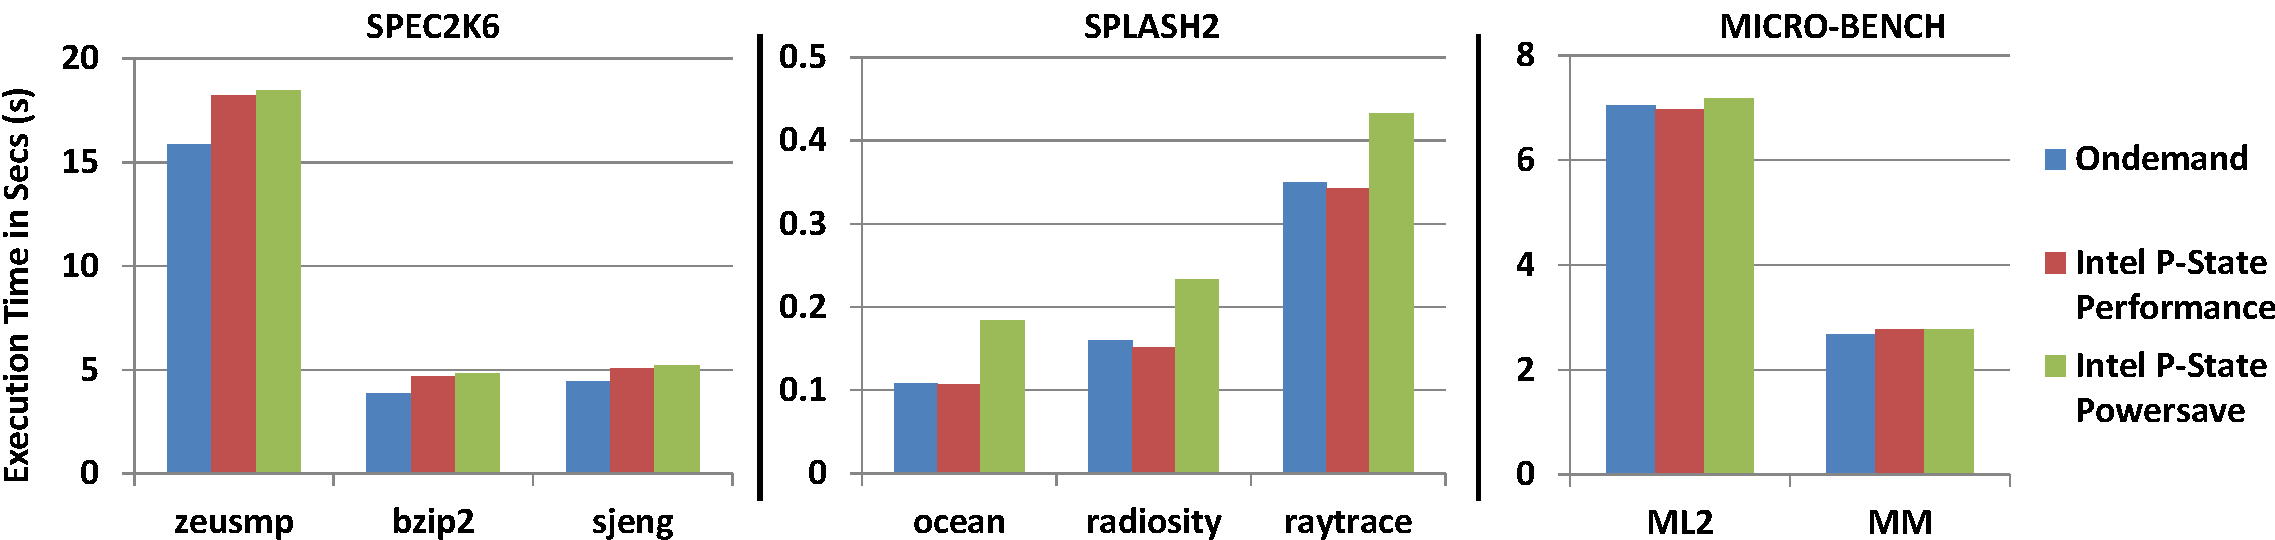
\includegraphics[width=\linewidth]{figs/def-exec-time-crop.pdf}
  \end{center}
  \vspace{-0.1in}
  \caption{Execution time for Linux ondemand and Intel P-state power governors}
  \label{fig:def-perf}
\end{figure*}

The case study in the previous section showed a contrived example and how cache misses are effected 
due to the imperfect frequency scaling in linux power governors.
In this section, we consider real applications and try to analyze how existing linux power
governors perform for different class of applications.

\subsection{Application categorization}
We chose applications from  SPEC2006~\cite{spec2006} and SPLASH2~\cite{splash2} to account for both single-threaded and 
multi-threaded applications' analysis. 
We also have written two micro-benchmarks which we call as MICRO-BENCH
suite from now, to exercise 
memory behavior. ML2 is a linked-list traversal workload and 
MM is a workload which has byte accesses larger than
cache line size. 
To first analyze the distribution of instruction in these applications,
we used the PIN~\cite{pin} binary instrumentation tool for profiling.
The PIN tool was modeled to account for total instructions in the application, 
instructions which get hit in the cache and instructions which miss in the cache
and actually access the memory. 
The application profiling was mainly done to figure out
which frequency must be scaled  
based on the time spent by these applications
in CPU or DRAM or Caches.
We could not get Disk (I/O) related instructions and I/O behavior
of applications, as PIN cannot model file system accesses, and
we have no control over the speed at which DISK accesses happen. So, our focus is
mainly on the following three categories:

\begin{itemize} 
\item \textit{Compute Intensive}: The applications which spend most of their execution
time in CPU core and have more computation instructions
between load/stores to the memory. For these applications, CPU
frequency is the important parameter.
\item \textit{Cache Sensitive}: The applications which have more memory access instructions,
but due to the locality of the data accesses, most of them get the data in CPU caches.
For these applications, again CPU frequency is important. 
For our analysis, we assume that, 
CPU cycles will be wasted in getting the data from the caches, whenever
it encounters load or store instructions. 
It is possible that just
by profiling the memory related instructions and not analyzing the cache accesses,
one could misinterpret the application as memory intensive always
and scale the DRAM frequency which we explain below. 
\item \textit{Memory Bound} These are the applications, which have lot of last level cache misses
and the accesses reach memory (DRAM). Increasing the CPU frequency for these applications could 
lead to wastage of energy and for better performance DRAM frequency might have to
be scaled rather than CPU frequency. 
\end{itemize}

Figure~\ref{fig:app-cat} shows the application categorization and distribution of instructions 
across seven SPEC2006 benchmarks, five SPLASH2 benchmarks and two micro-benchmarks. 
We see that SPEC2006 has more compute intensive instructions with some of them
having good cache locality. SPLASH2 has more cache sensitive instructions 
in average with some having good percentage of compute as well as memory related instructions. 
The micro-benchmark MM has lot of cache related instructions and many accessing memory.
ML2 has zero cache access and all of the load/store  instructions access the memory.

\subsection{Power governors performance}

We executed these applications on a Linux kernel with Ondemand~\cite{ondemand2006} power governor
as the default and also ran the applications on two power governors (performance and powersave) 
of Intel's recent P-state~\cite{pstate, rotem2012power} driver \footnote{
Section~\ref{sec:meth} explains the methodology used for performance and energy estimation}. 
We considered Intel's P-state driver, as it has access to turbo boost frequency 
through direct driver interface. Figure~\ref{fig:def-perf} shows the execution time 
of selected benchmarks across all three applications suites (SPEC2K6, SPLASH2 and MICRO-BENCH) for
three discussed power governors. It is seen that, each of the three power governors 
have similar performance even though each has a distinct objective.
Intel P-state performance governor is supposed to boost the performance
with access to turbo boost frequency. Even though, P-state powersave governor 
has slightly worst performance compared to other two, as it tries
to save power by reducing the frequency, the difference is not significant.
The next subsection details on energy efficiency of each of these governors. 

\subsection{Power governors energy efficiency}
\begin{figure}[h]
  \begin{center}
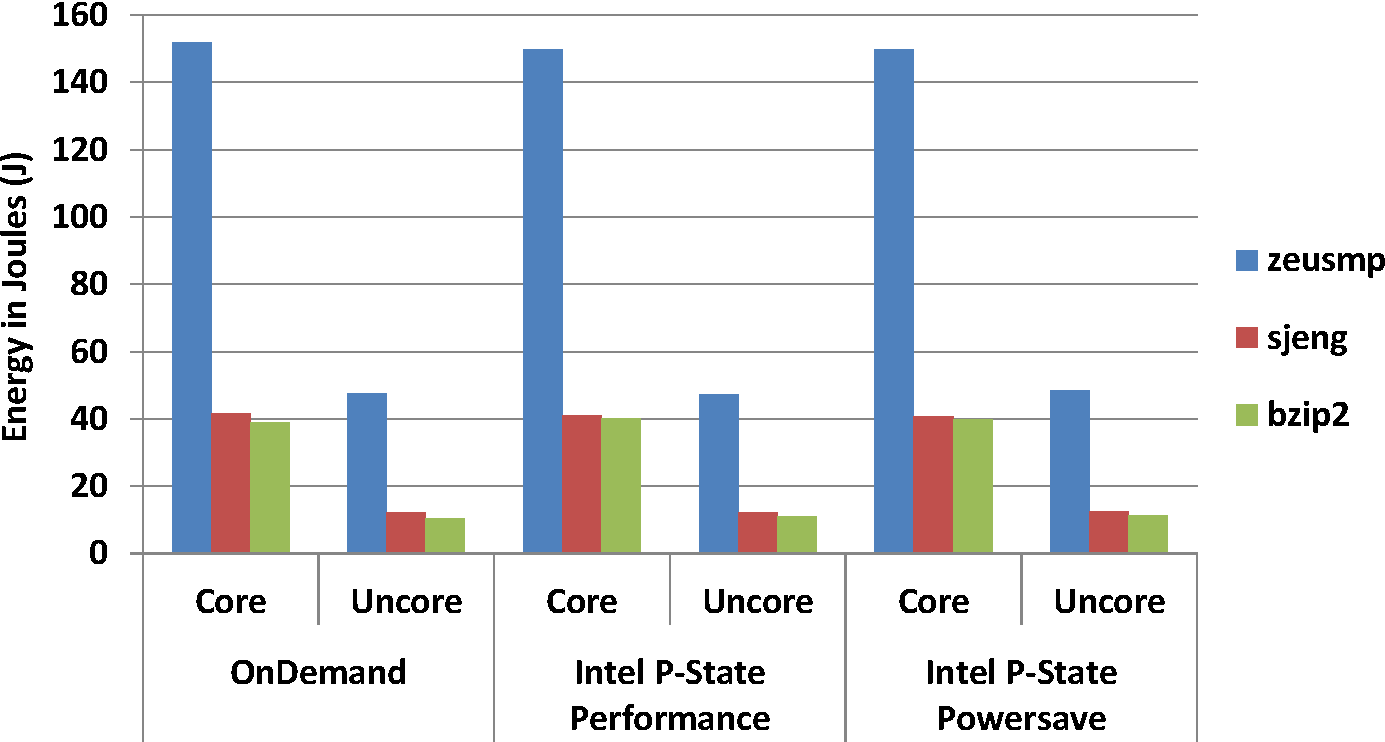
\includegraphics[width=\linewidth]{figs/def-drivers-spec-crop.pdf}
  \end{center}
  \vspace{-0.1in}
  \caption{Energy Consumption for SPEC2006 workloads with ondemand and p-state governors}
  \label{fig:spec-energy}
\end{figure}

As seen with the execution time, we also wanted to analyze
if the power governors perform similar with respect to energy efficiency.
Figure~\ref{fig:spec-energy} shows the energy consumption in Joules for three of the SPEC 2006
benchmarks. We see that the core and encore energy for all the three 
benchmarks across all three governors are similar.  
Figure~\ref{fig:micro-energy} shows similar trend for memory intensive micro-benchmarks.


\begin{figure}[h]
  \begin{center}
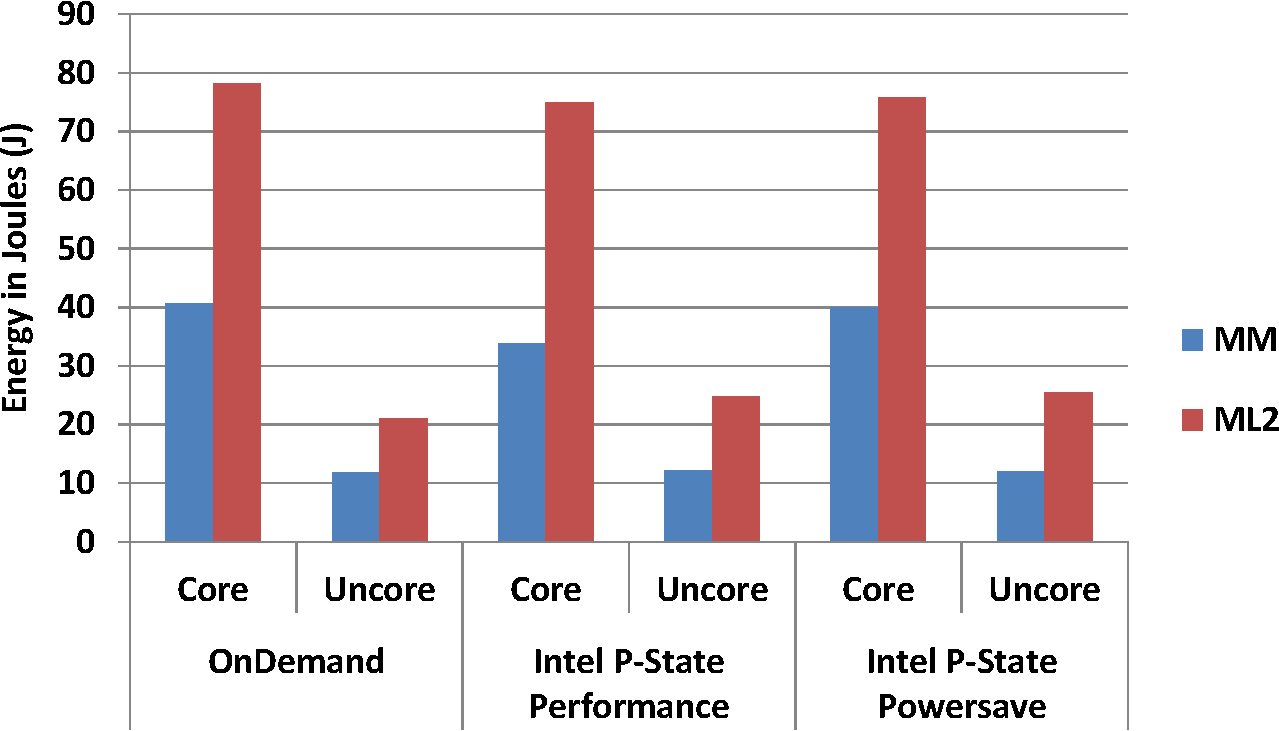
\includegraphics[width=\linewidth]{figs/def-drivers-micro-crop.pdf}
  \end{center}
  \vspace{-0.1in}
  \caption{Energy Consumption for MICRO-BENCH with ondemand and p-state governors}
	\label{fig:micro-energy}
\end{figure}

Figure~\ref{fig:splash-energy} shows energy consumption for SPLASH2 benchmarks.
In case of SPLASH2 benchmarks, it can be seen that for all three workloads, P-state powersave saves more
energy around 2-3 joules compared to other two governors. This complements
why powersave governor had worst execution time than other two. However, still 
the powersave governor does not save significant energy savings even though it reduces 
the CPU frequency to save lot of power.

\begin{figure}[h]
  \begin{center}
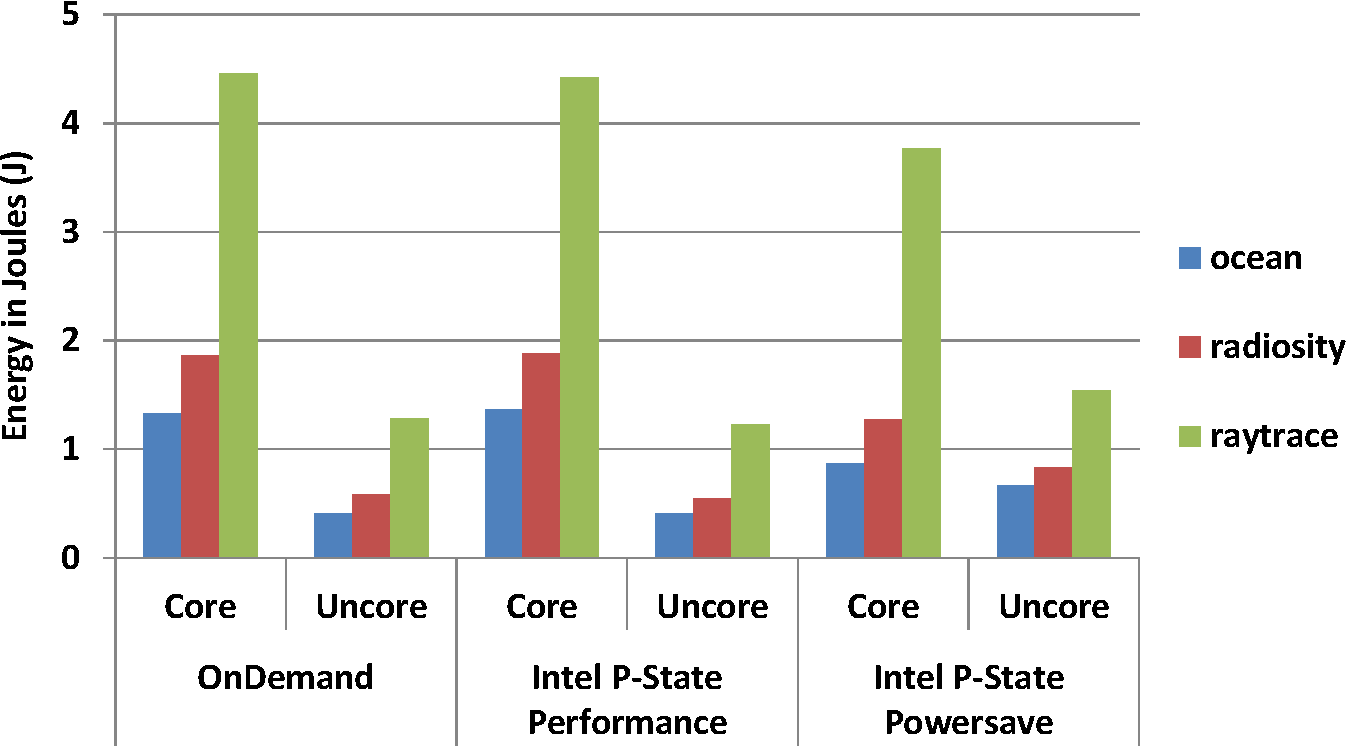
\includegraphics[width=\linewidth]{figs/def-drivers-splash-crop.pdf}
  \end{center}
  \vspace{-0.1in}
  \caption{Energy Consumption for SPLASH2 workloads with ondemand and p-state governors}
  \label{fig:splash-energy}
\end{figure}

\vspace{-0.1in}
The takeaway from this analysis is that: 1) existing linux power governors 
are optimized only for compute intensive benchmarks;
2) All the three power governors mainly use "race to halt" approach to execute workloads 
fast (scale CPU frequency) and thus save energy;
3) The existing power governors are not application-aware and do not rely
on application characteristics to scale CPU or DRAM frequency;
4) ondemand governor scales frequency on overall system load
rather than individual application requirements;
Based on these takeaways, we believe that Operating systems
should give more freedom to user-space for energy management
and making better policy decisions. User-space has more 
information about applications it is running than
the underlying drivers or hardware.
We now present our model E-MOS, which is an application-aware
energy management model and discuss its implications on OS energy management polices.
